\documentclass[border=6pt]{standalone}
\usepackage{amsmath,amssymb}
\usepackage{tikz}
\usetikzlibrary{arrows.meta,positioning,fit,backgrounds,calc}

\definecolor{cbblue}{HTML}{2A78D6}
\definecolor{cbviolet}{HTML}{4A3AA7}
\definecolor{cbaqua}{HTML}{1BAF7A}
\definecolor{cbred}{HTML}{E34948}
\definecolor{cbink}{HTML}{26251F}
\definecolor{cbmuted}{HTML}{898781}

\begin{document}
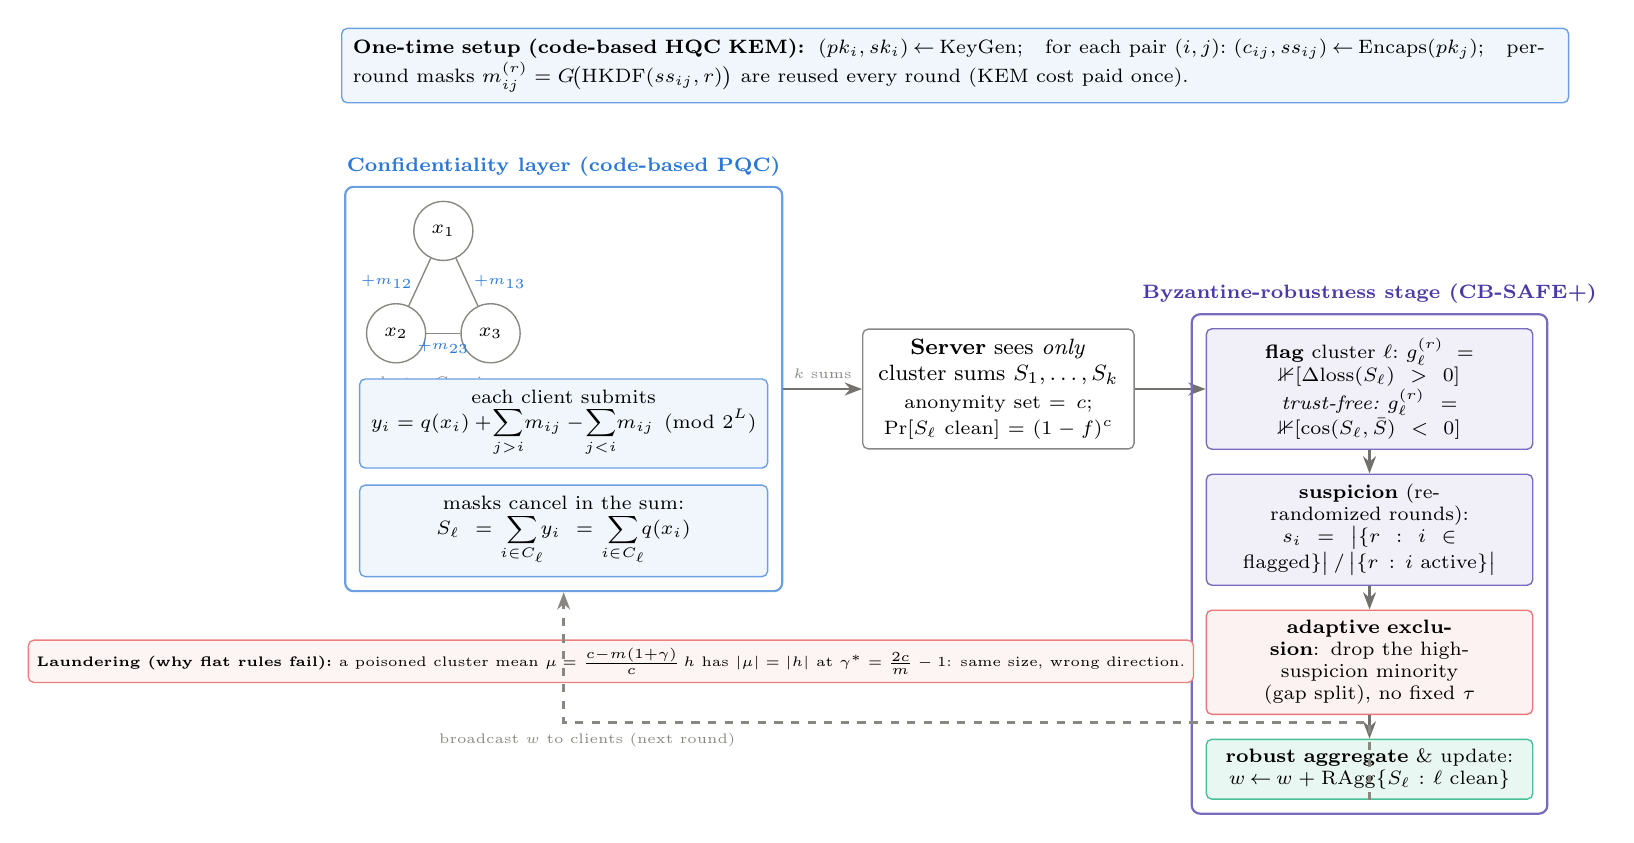
\begin{tikzpicture}[
  >={Stealth[length=2.2mm]},
  font=\footnotesize, line width=0.5pt, node distance=5mm,
  client/.style={circle,draw=cbmuted,fill=white,minimum size=7.5mm,inner sep=0pt,font=\scriptsize},
  op/.style={rounded corners=2pt,draw=cbink!55,fill=white,align=center,inner sep=3.5pt},
  eq/.style={rounded corners=2pt,draw=cbblue!70,fill=cbblue!7,align=center,inner sep=4pt},
  vio/.style={rounded corners=2pt,draw=cbviolet!75,fill=cbviolet!8,align=center,inner sep=3.5pt},
  aqua/.style={rounded corners=2pt,draw=cbaqua!80,fill=cbaqua!10,align=center,inner sep=3.5pt},
  flow/.style={->,draw=cbink!65,line width=0.9pt},
]

% ================= SETUP RIBBON =================
\node[eq, align=left, text width=15.3cm, font=\scriptsize] (setup) at (7.1,5.5) {%
\textbf{One-time setup (code-based HQC KEM):}\;
$(pk_i,sk_i)\!\leftarrow\!\mathrm{KeyGen}$;\quad
for each pair $(i,j)$:\ $(c_{ij},ss_{ij})\!\leftarrow\!\mathrm{Encaps}(pk_j)$;\quad
per-round masks $m_{ij}^{(r)}=G\!\big(\mathrm{HKDF}(ss_{ij},r)\big)$ are reused every round (KEM cost paid once).};

% ================= STAGE 1: cluster + masking =================
\node[client] (c1) at (0.6,3.4) {$x_1$};
\node[client] (c2) at (0.0,2.1) {$x_2$};
\node[client] (c3) at (1.2,2.1) {$x_3$};
\draw[cbmuted] (c1)--(c2) node[midway,left=-1pt,font=\tiny,cbblue]{$+m_{12}$};
\draw[cbmuted] (c1)--(c3) node[midway,right=-1pt,font=\tiny,cbblue]{$+m_{13}$};
\draw[cbmuted] (c2)--(c3) node[midway,below=-1pt,font=\tiny,cbblue]{$+m_{23}$};
\node[font=\tiny,cbmuted] at (0.6,1.45) {cluster $C_\ell$, size $c$};

\node[eq, below=3mm of c2.south west, anchor=north west, xshift=-2mm, text width=4.9cm, font=\scriptsize] (mask) {%
each client submits\\[1pt]
$y_i=q(x_i)+\!\displaystyle\sum_{j>i}\!m_{ij}-\!\sum_{j<i}\!m_{ij}\pmod{2^{L}}$};

\node[eq, below=2mm of mask, text width=4.9cm, font=\scriptsize] (sum) {%
masks cancel in the sum:\\[1pt]
$S_\ell=\!\!\displaystyle\sum_{i\in C_\ell}\!\! y_i=\!\!\sum_{i\in C_\ell}\!\! q(x_i)$};

\node[draw=cbblue!70,rounded corners=3pt,thick,fit=(c1)(c2)(c3)(mask)(sum),inner sep=5pt,label={[cbblue,font=\scriptsize\bfseries]above:Confidentiality layer (code-based PQC)}] (conf) {};

% ================= STAGE 2: server sees only sums =================
\node[op, right=10mm of conf, text width=3.2cm, align=center] (server) {%
\textbf{Server} sees \emph{only}\\ cluster sums $S_1,\dots,S_k$\\[2pt]
{\scriptsize anonymity set $=c$;\\ $\Pr[S_\ell\text{ clean}]=(1-f)^c$}};
\draw[flow] (conf.east) -- (server.west) node[midway,above,font=\tiny,cbmuted]{$k$ sums};

% ================= STAGE 3: CB-SAFE+ =================
\node[vio, right=9mm of server, text width=3.9cm, font=\scriptsize] (flag) {%
\textbf{flag} cluster $\ell$:\ $g_\ell^{(r)}=\mathbb{1}[\Delta\mathrm{loss}(S_\ell)>0]$\\
\emph{trust-free:}\ $g_\ell^{(r)}=\mathbb{1}[\cos(S_\ell,\bar S)<0]$};
\node[vio, below=3mm of flag, text width=3.9cm, font=\scriptsize] (susp) {%
\textbf{suspicion} (re-randomized rounds):\\
$s_i=\big|\{r: i\in\text{flagged}\}\big|\,/\,\big|\{r: i\text{ active}\}\big|$};
\node[aqua, below=3mm of susp, text width=3.9cm, font=\scriptsize, draw=cbred!75, fill=cbred!7] (excl) {%
\textbf{adaptive exclusion}: drop the high-\\ suspicion minority (gap split), no fixed $\tau$};
\node[aqua, below=3mm of excl, text width=3.9cm, font=\scriptsize] (ragg) {%
\textbf{robust aggregate} \& update:\\
$w\!\leftarrow\! w+\mathrm{RAgg}\{S_\ell:\ell\text{ clean}\}$};
\draw[flow] (flag)--(susp);  \draw[flow] (susp)--(excl);  \draw[flow] (excl)--(ragg);
\draw[flow] (server.east) |- (flag.west);
\node[draw=cbviolet!75,rounded corners=3pt,thick,fit=(flag)(susp)(excl)(ragg),inner sep=5pt,label={[cbviolet,font=\scriptsize\bfseries]above:Byzantine-robustness stage (CB-SAFE+)}] (rob) {};

% laundering callout
\node[rounded corners=2pt,draw=cbred!70,fill=cbred!6,align=left,inner sep=3pt,font=\tiny,
      below=6mm of conf.south, anchor=north, xshift=6mm] (laund) {%
\textbf{Laundering (why flat rules fail):}\ a poisoned cluster mean
$\mu=\frac{c-m(1+\gamma)}{c}\,h$ has $|\mu|=|h|$ at $\gamma^\ast=\tfrac{2c}{m}-1$: same size, wrong direction.};

% broadcast loop
\draw[flow,dashed,draw=cbmuted] (ragg.south) |- ($(laund.south)+(0,-0.5)$) -| node[near start,below,font=\tiny,cbmuted]{broadcast $w$ to clients (next round)} (conf.south);

\end{tikzpicture}
\end{document}
